\documentclass{article}
\usepackage{graphicx}
\usepackage[margin=0.75in]{geometry}
\begin{document}
\title{BIOS 611 Final Project}
\author{Yixiang Qu \\ e-mail: yqu@unc.edu}
\date{October 28, 2021}
\maketitle

\section{Introduction}
With progress on both the theoretical and the computational fronts the use of spline modelling has become an established tool in statistical regression analysis. In particular, splines are regularly used for building explanatory models in clinical research. Indeed, many new methodological developments in modern biostatistics make use of splines to model smooth functions of interest, including e.g. non-linear effects of continuous covariates, avoiding distributional assumptions and modelling time-dependent effects in survival analysis, time series, cumulative effects and frequency distributions.
\section{Different spline methods}
\subsection{Thin plate regression spline}
\begin{figure*}[h]
    \centering
    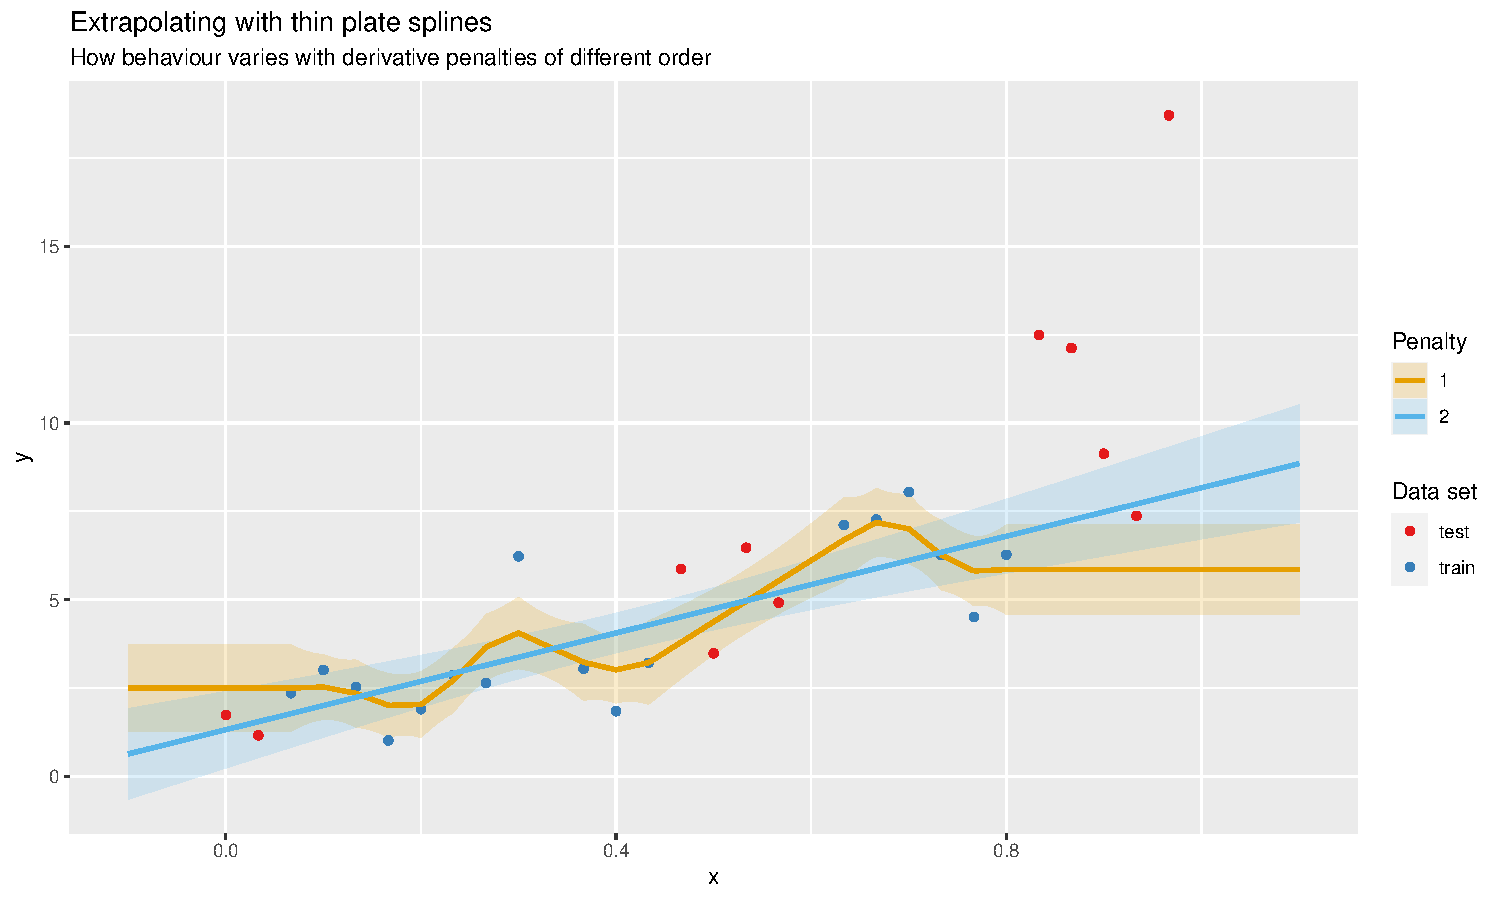
\includegraphics[width=0.9\textwidth]{figure/tprs.pdf}
    \caption{Results of thin plate regression spline}
    \label{tprs}
    \end{figure*}

\subsection{B spline}
\begin{figure*}[h]
    \centering
    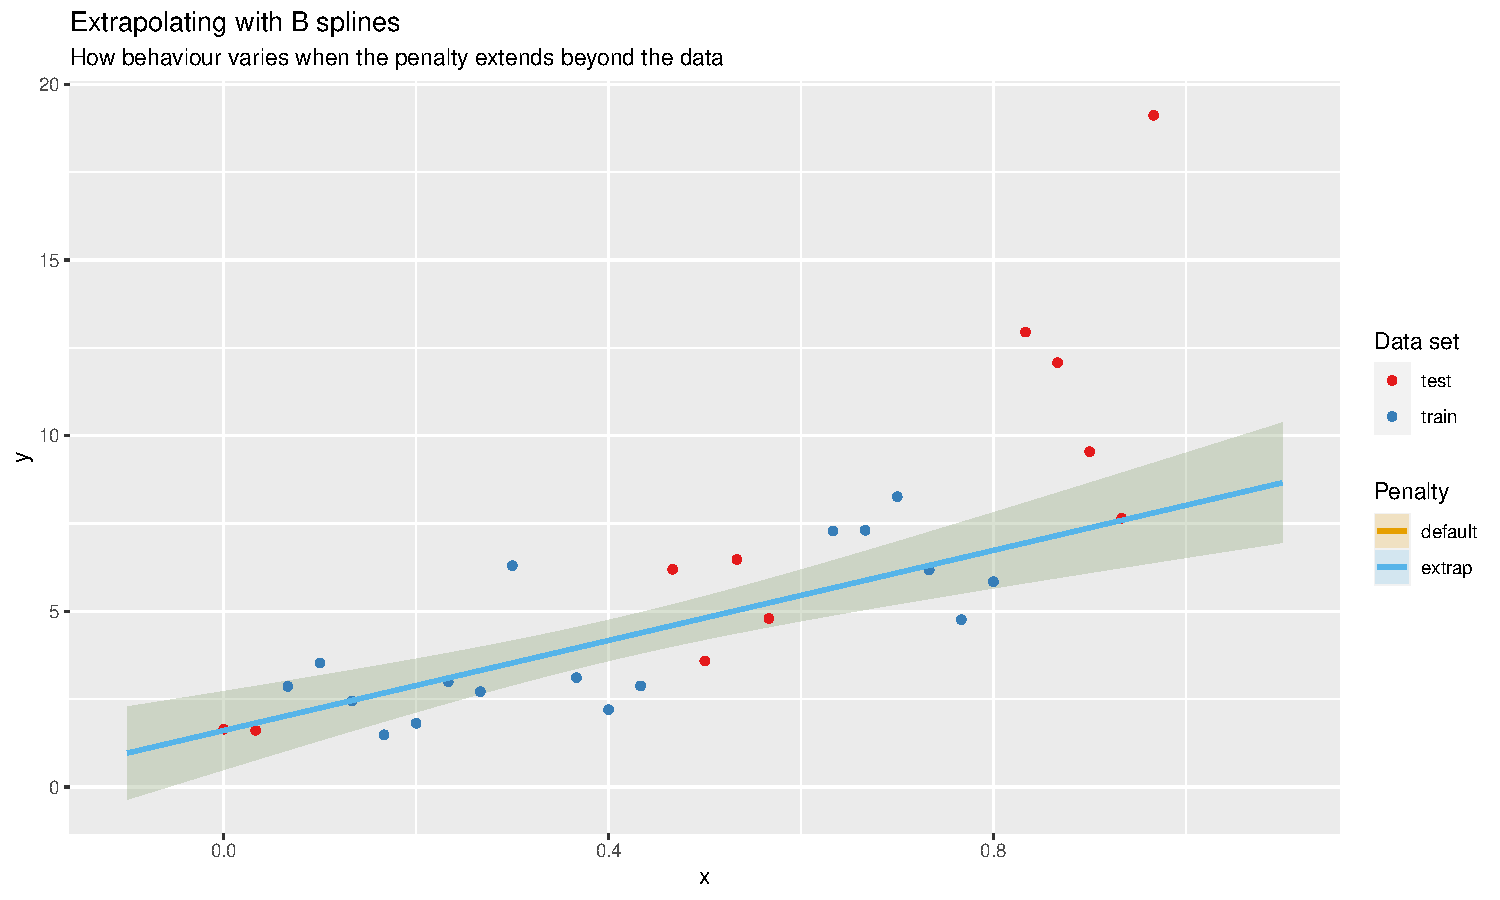
\includegraphics[width=0.9\textwidth]{figure/B_spline.pdf}
    \caption{Results of B spline}
    \label{bs}
    \end{figure*}

\end{document}